\documentclass[11pt]{article}
\usepackage{graphicx}
\graphicspath{ {images/} }
\usepackage[margin=0.75in]{geometry}

\title{Working Memory Related Brain Network Connectivity in Individuals with Schizophrenia and Their Siblings}
\author{
  Li, Jie\\
  \texttt{Jay4869}
  \and
  Li, Zeyu\\
  \texttt{lizeyuyuz}
  \and
  Yun, Chuan\\
  \texttt{ay2456}
  \and
  Zhang, Qiangyuan\\
  \texttt{amandazhang}
}

\bibliographystyle{siam}

\begin{document}
\maketitle

\abstract{A recent study shows that schizophrenia reflects a ``dysconnection'' syndrome, which means schizophrenia can result in damaging functional brain connectivity in neural networks. We are interested in schizophrenia, so we decide to look into their studies to see if their conclusion makes sense. Therefore, we download the data they got during their tests and redo their analysis by following their steps in the paper. Even though we aren't able to go through all the analysis they did, we expect to get the same result for the analysis we do.}

\section{Introduction}

Schizophrenia is a chronic, severe, and disabling brain disorder that has affected people throughout history. Or you can just think it as an illness that causes abnormal social behavior and failure to recognize what is real. Previous studies showed that changes in the function of a single brain region, or even a brain system, cannot explain the functional impairments seen in this illness. This means that the causes of schizophrenia is much more complicated than we think. A recent study shows that individuals with schizophrenia have reduced connectivity between neural networks, which could be a forward step to solve the cause of this illness.

The paper suggests this conclusion is ``Working memory related brain network connectivity in individuals with schizophrenia and their siblings'' \cite{schizophreniabrainconnectivity}, and the data they used is available on OpenFMRI.org under ``Working memory in healthy and schizophrenic individuals''. The paper thinks that neural networks which are critical for cognitive function might be affected by schizophrenia, because individuals with schizophrenia have severe cognitive issues. In particular, these neural networks are (1) Dorsal fronto-parietal network (FP), (2) Cingulo-opercular network (CO), (3) Cerebellar network (CER) and (4) ``Default mode'' network (DMN) and they are the regions of interest (ROIs) for this paper. They showed that individuals with schizophrenia have reduced connectivity between neural networks.

In total 102 participants in the paper's experiment and they were divided into 4 groups: (1) individuals with Schizophrenia (SCZ; N = 19); (2) the siblings of individuals with schizophrenia (SCZ-SIB; N = 28); (3) healthy controls (CON; N = 10); and (4) the siblings of healthy controls (CON-SIB; N = 17). In order to assessing functional brain connectivity, they used blood oxygen level dependent (BOLD) time series acquired using fMRI. 

The paper's objective is finding connectivity within and between each ROI on different tasks. They extracted these ROIs and worked directly on them. Since we do not have the knowledge about partition the brain into ROIs, we could not do the same analysis as them. Therefore, we will simply focus on the entire brain and find the region related to these tasks. Also, they worked on all subjects and did comparisons between different groups. Since we don't have time to go through all of the subjects, we choose the first subject from SCZ group. If we have time, we will work on another subject from CON group and do a comparison between these two.

Our goal is to use the paper's data to do some statistical analysis, and see if our analysis could come up with the same conclusion as the paper. We understand the fact that we couldn't reproduce the whole analysis part of the paper due to the limitation of knowledge and time. However, with the analysis we designed for this data, we will finally get a great result.

%You should explain the basic idea of the paper in a paragraph.  You should also perform basic sanity check on the data
%(e.g., can you downloaded, can you load the files, confirm that you have the correct number of subjects).
%Briefly explain what reproducibility means and in what sense you will try to reproduce this study.

\section{Data}

We went to OpenFMRI.org and looked through all the files it has for this paper. The are many data files grouped by subjects and we only downloaded ``ds115-sub001-005.tg'', which contains the brain image of the first five subjects, and the ``ds115-metadata.tg'', which contains metadata for the paper. Since we only chose one subject, which is sub001, we only need his part in the data file. 

First, we checked all the files for sub001 and found there are three tasks for our subject. We realized that these were ``N - back'' working memory task in the paper. This task was to respond for each letter shown whether it was the same as a pre-specified letter (0-back), the same as the immediately preceding letter (1-back), or the same as the letter shown two trials previously (2-back). For our subject, there were three BOLD runs, each consisting of two blocks of 0-back, 1-back, or 2-back working memory task. 

Second, we found that under each task there are four brain images. We thought one of them should be the raw image and the others were some-how processed by the authors. Therefore, we plotted these four brain images and chose the most blurred one (This is probably because it is after smoothing), which is ``BOLD-mcf-brain.nii''. 

Then, similar to what we did in class, we used HRF function to convolve our neural prediction, This will give us a hemodynamic prediction, under the linear-time-invariant assumptions of the convolution. This is a very important step because we will use convolution data in our linear modeling process in the future. Here is the comparison between the original neural prediction and convolved.

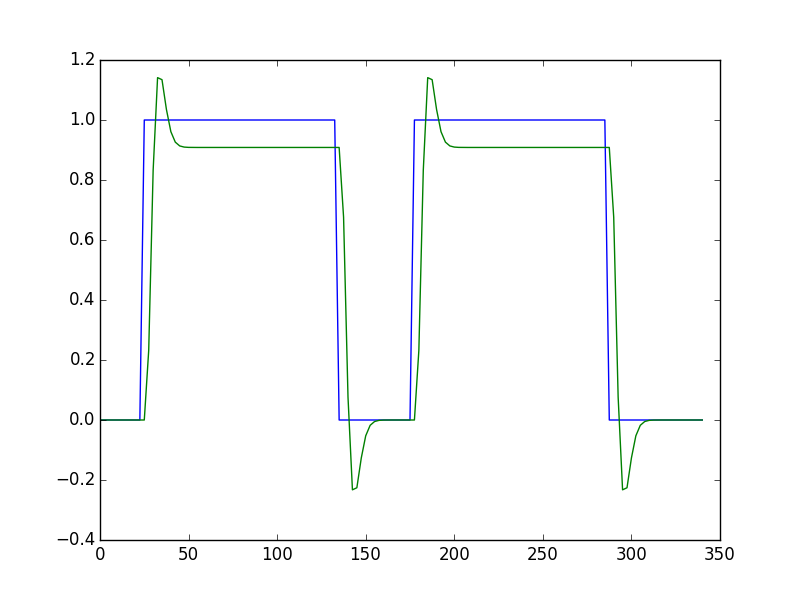
\includegraphics{task001_run001_conv005}

\section{Methods}
\section{Results}
\section{Discussion}


\bibliography{project}

\end{document}
